\section{Sensing Challenges}
\label{sec:sensing-challenges}

With vehicle identities being discovered by traffic cameras along their moving trajectories, a straightforward solution is to maintain such identities across all roadways and reconstruct the trajectory of each vehicle by concatenating its sequence of timestamped observations from all related traffic cameras. 
The camera sensing network's intrinsic incompleteness and inaccuracy make it difficult to implement this system in practice.
Traffic camera observations are incomplete, as not all road intersections are covered, leading to uncertainty in inferring moving trajectories in uncovered areas.
Vehicle identities extracted from video and image analysis may be inaccurate due to camera and data quality heterogeneity between different cameras that also have different views (e.g., front-view vs. rear-view), angles, focus, and environmental conditions.
Low-quality video data can lead to severe issues in vehicle identification using the latest \ac{lpr} or \ac{re-id} methods \cite{zhou2018aware}.
\Cref{fig:vehicle-identity-uncertainty}(a) represents how it is hard to detect license plates when the images are blurry, the license is dirty, part of the license is not shown in the image because it is hidden by other objects or cut from the image, or there are difficult lighting conditions, respectively, from left to right.
More over, \Cref{fig:vehicle-identity-uncertainty}(b) shows how different vehicles can have similar appearances.
Finally, \Cref{fig:vehicle-identity-uncertainty}(c) shows that different angles and lighting conditions can help mislead the identification of the same vehicle.

\begin{figure}
\centering
  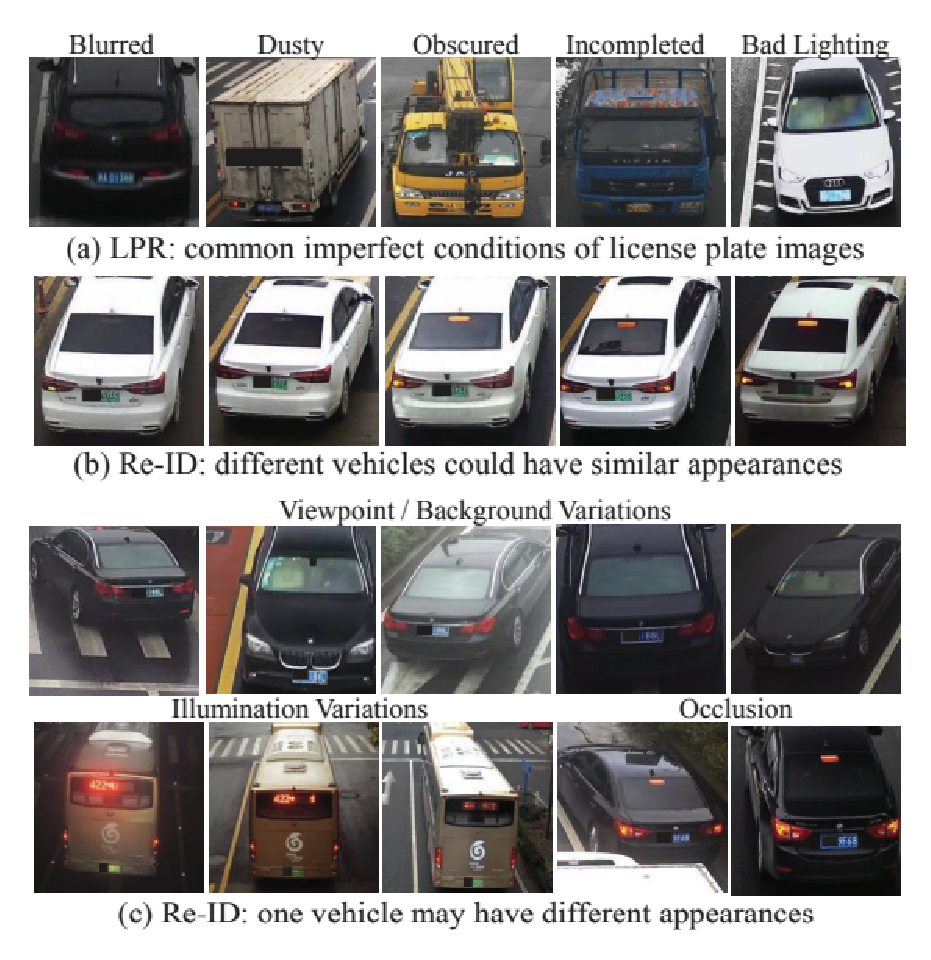
\includegraphics[width=0.9\linewidth]{figures/difficulty-in-identifying-vehicles.eps}
  \caption{vehicle's identity uncertainties \cite{tong2021large}}
  \label{fig:vehicle-identity-uncertainty}
  %\vspace{-5mm}
\end{figure}

Other difficulties can hinder the accuracy of the generated vehicle trajectories, such as false positives as presented in \Cref{fig:false-positives}.
Furthermore, uncertainties will happen because of the miclassification of one or more digits of the license plate, which will cause the vehicle to be identified as a different car as depicted in \Cref{fig:license-misclassification}.
Additionally, there are uncertainties due to the lack of cameras at some intersections.
After the analysis of the road network, it is depicted that only 57\% of intersections are covered with cameras.

\begin{figure}
\centering
  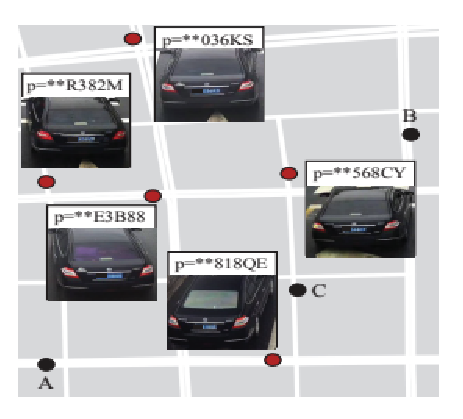
\includegraphics[width=0.5\linewidth]{figures/false-positives.eps}
  \caption{\ac{re-id} false positives \cite{tong2021large}}
  \label{fig:false-positives}
  %\vspace{-5mm}
\end{figure}

\begin{figure}
\centering
  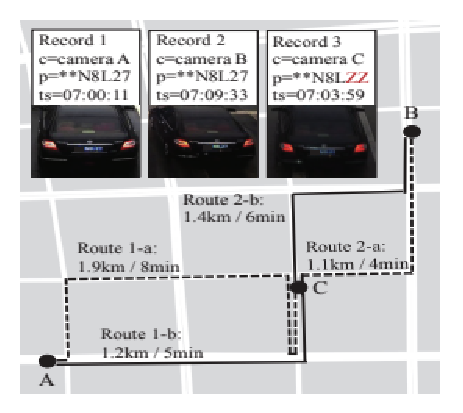
\includegraphics[width=0.5\linewidth]{figures/license-misclassification.eps}
  \caption{\ac{re-id} due to license misclassification \cite{tong2021large}}
  \label{fig:license-misclassification}
  %\vspace{-5mm}
\end{figure}